\documentclass[12pt]{article}
\usepackage{float}
\usepackage[dvipsnames]{xcolor}
\usepackage{dingbat, tikz}
\usepackage{amsfonts,amsmath, color, fullpage, graphicx, mathtools, empheq, amsthm, amssymb}
\usepackage{wasysym}
\usepackage{thmtools}
\usepackage{listings}
\usepackage[framed]{mcode}

%To allow for matrix larger than 10x10
\setcounter{MaxMatrixCols}{11}

%To set thumbs up as QED symbol
\renewcommand{\qedsymbol}{\begingroup \color{blue} \rightthumbsup \endgroup}

%To make a new command for an asterisk in a circle
\newcommand{\circlesign}[1]{ 
    \mathbin{
        \mathchoice
        {\buildcirclesign{\displaystyle}{#1}}
        {\buildcirclesign{\textstyle}{#1}}
        {\buildcirclesign{\scriptstyle}{#1}}
        {\buildcirclesign{\scriptscriptstyle}{#1}}
    } 
}
\newcommand\buildcirclesign[2]{%
    \begin{tikzpicture}[baseline=(X.base), inner sep=0, outer sep=0]
    \node[draw,circle] (X)  {\ensuremath{#1 #2}};
    \end{tikzpicture}%
}

%To use a border matrix with brackets
\usepackage{etoolbox}
\let\bbordermatrix\bordermatrix
\patchcmd{\bbordermatrix}{8.75}{4.75}{}{}
\patchcmd{\bbordermatrix}{\left(}{\left[}{}{}
\patchcmd{\bbordermatrix}{\right)}{\right]}{}{}



\def\C{\mathbb{C}}
\def\N{\mathbb{N}}
\def\Q{\mathbb{Q}}
\def\R{\mathbb{R}}
\def\Ts{\mathbb{T}}
\def\Z{\mathbb{Z}}
\def\T{\mathcal{T}}
\def\P{\mathcal{P}}
\title{\underline{Math 226B: Homework \#2}}
\author{\huge Kara Gorman}
\begin{document}
\maketitle


\bigskip\bigskip
\noindent
\textbf{Problem 1:}

\begin{itemize}

\item[(a)] For $A = \text{make\_2d\_laplacian(m)}$, and $m = m_0 := 67$, compute the Cholesky factor $L$ of $A$ for the following five cases, and report the number of nonzero entries of $L$, and a plot of the sparsity structure of $L$.

\begin{figure}[H]
\center
\caption{2D Cholesky Sparsity Structure}
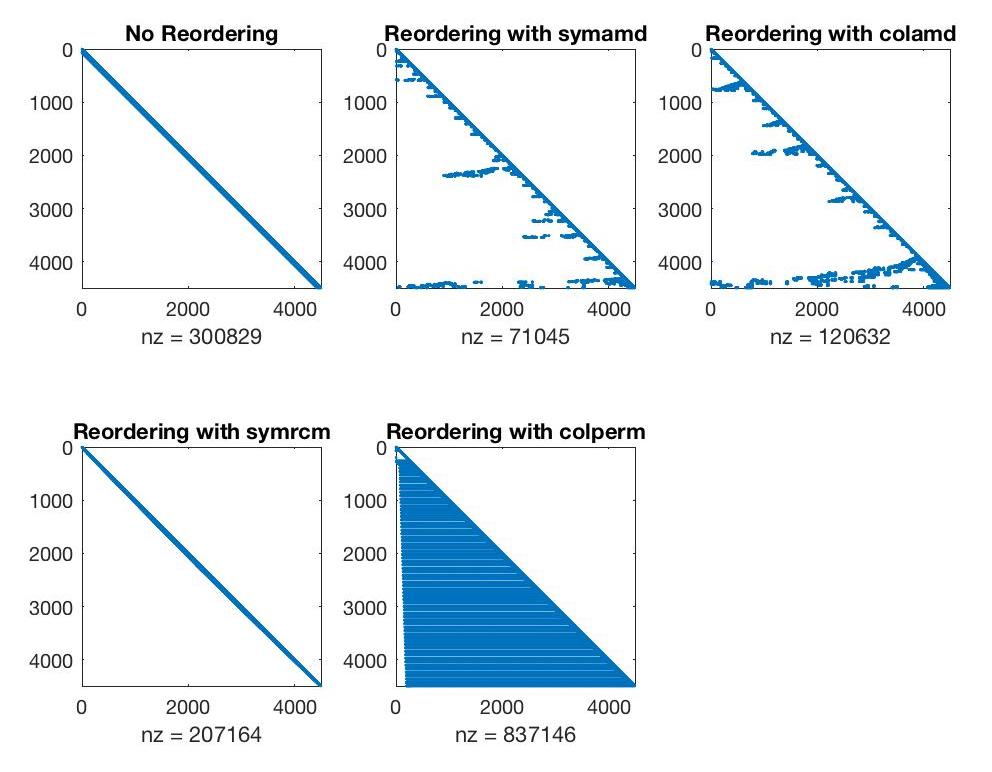
\includegraphics[scale=.4]{2d_laplacian_graphs.jpg}
\caption{2D Cholesky Sparsity Structure}
\end{figure}

\item For $m = 2^i m_0$, $i = 0,1,2, \dots$, compute the Cholesky factor $L$ of $A$ using the symamd ordering.  As $i$ increases, you will run out of storage or CPU time.  For which $i$ does this happen on the machine you run Matlab on?\\

\lstset{language=matlab,frame=single}
\begin{lstlisting}[caption=Matlab Code to for when 2D Cholesky Quits]
m0 = 67;
i = 0;

while (i >= 0)
    m = (2^i)*m0;
    i = i + 1
    A = make_2d_laplacian(m);
    p = symamd(A);
    L = chol(A(p,p),'lower');
end
\end{lstlisting}

\underline{Result:} Matlab crashed during the iteration corresponding to $i = 7$.\\
\qed


\item[(b)] For $A = \text{make\_3d\_laplacian(m)}$, and $m = m_0 := 37$, compute the Cholesky factor $L$ of $A$ for the following five cases, and report the number of nonzero entries of $L$, and a plot of the sparsity structure of $L$.

\begin{figure}[H]
\center
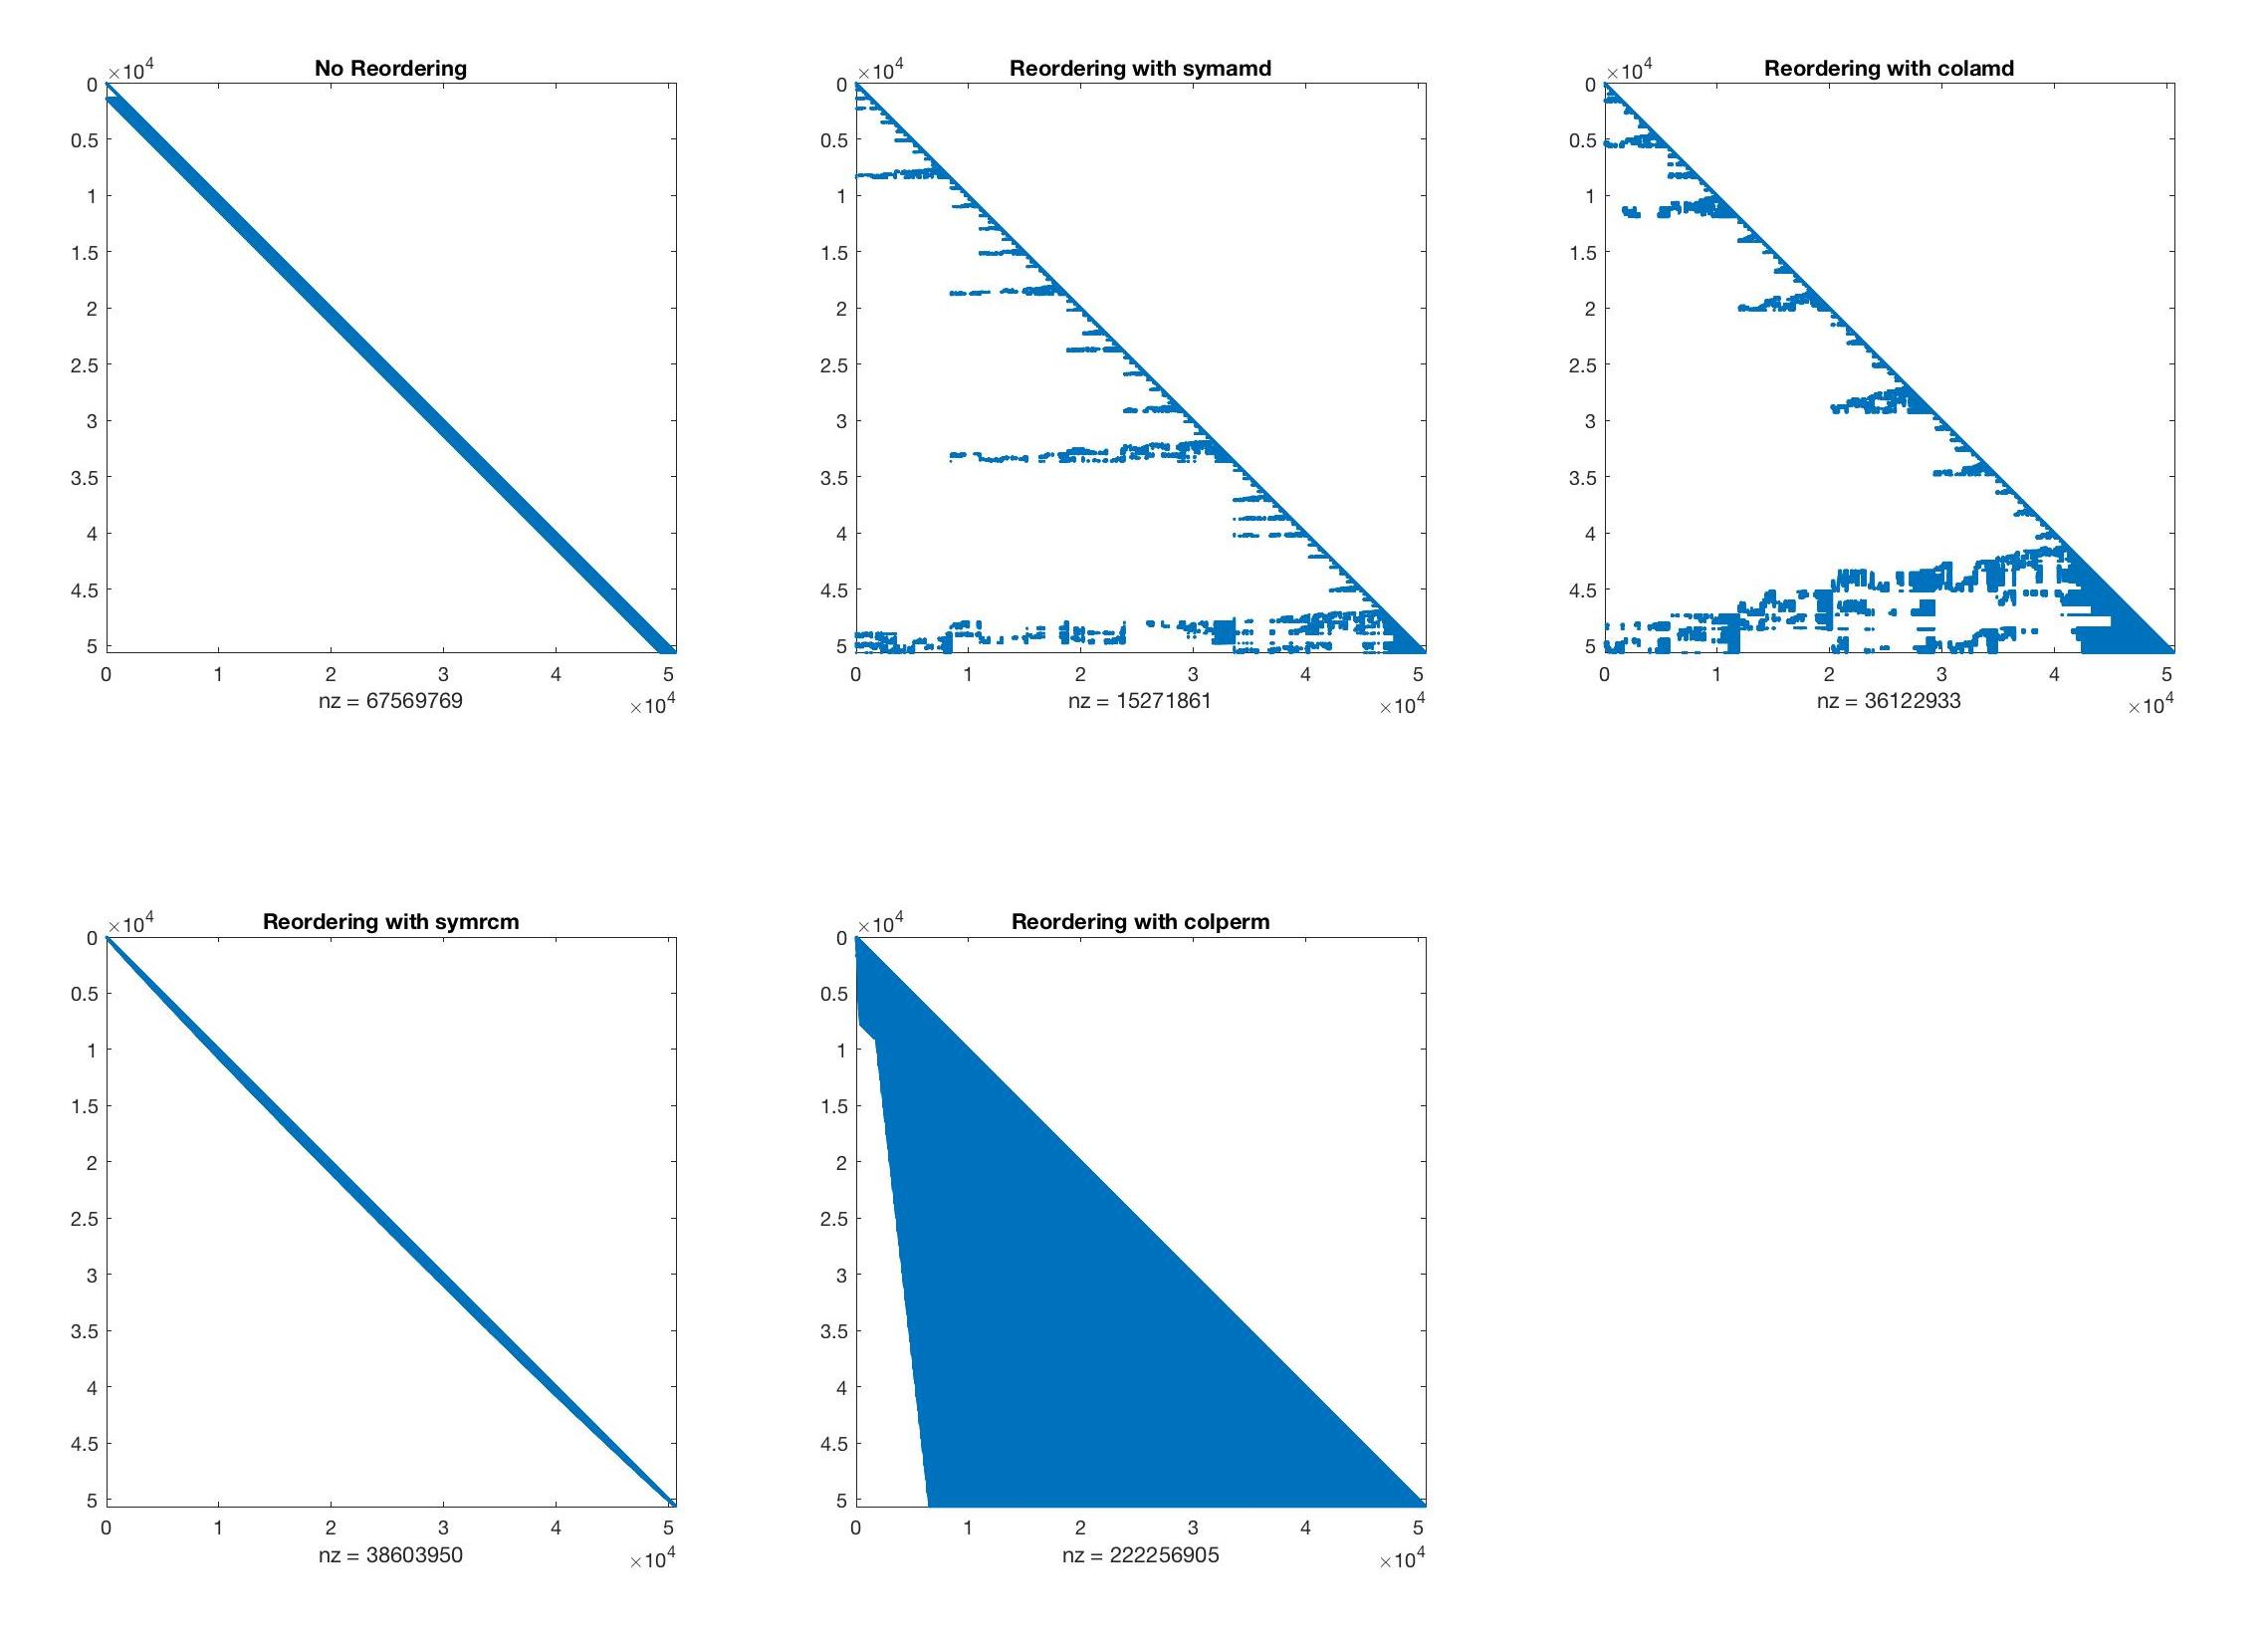
\includegraphics[scale=.16]{3d_laplacian_graphs.jpg}
\caption{3D Cholesky Sparsity Structure}
\end{figure}

\item For $m = 2^i m_0$, $i = 0,1,2, \dots$, compute the Cholesky factor $L$ of $A$ using the symamd ordering.  As $i$ increases, you will run out of storage or CPU time.  For which $i$ does this happen on the machine you run Matlab on?\\

\lstset{language=matlab,frame=single}
\begin{lstlisting}[caption=Matlab Code to for when 3D Cholesky Quits]
m0 = 37;
i = 0;

while (i >= 0)
    m = (2^i)*m0;
    i = i + 1
    A = make_3d_laplacian(m);
    p = symamd(A);
    L = chol(A(p,p),'lower');
end
\end{lstlisting}

\underline{Result:} Matlab crashed during the iteration corresponding to $i = 3$.\\
\qed
\end{itemize}


\bigskip\bigskip
\noindent
\textbf{Problem 2:}  You are given a $9 \times 9$ matrix $A \succ 0$ with the given sparsity structure.\\

\begin{itemize}

\item[(a)] Show the graph associated with $A$.\\

\begin{figure}[H]
\center
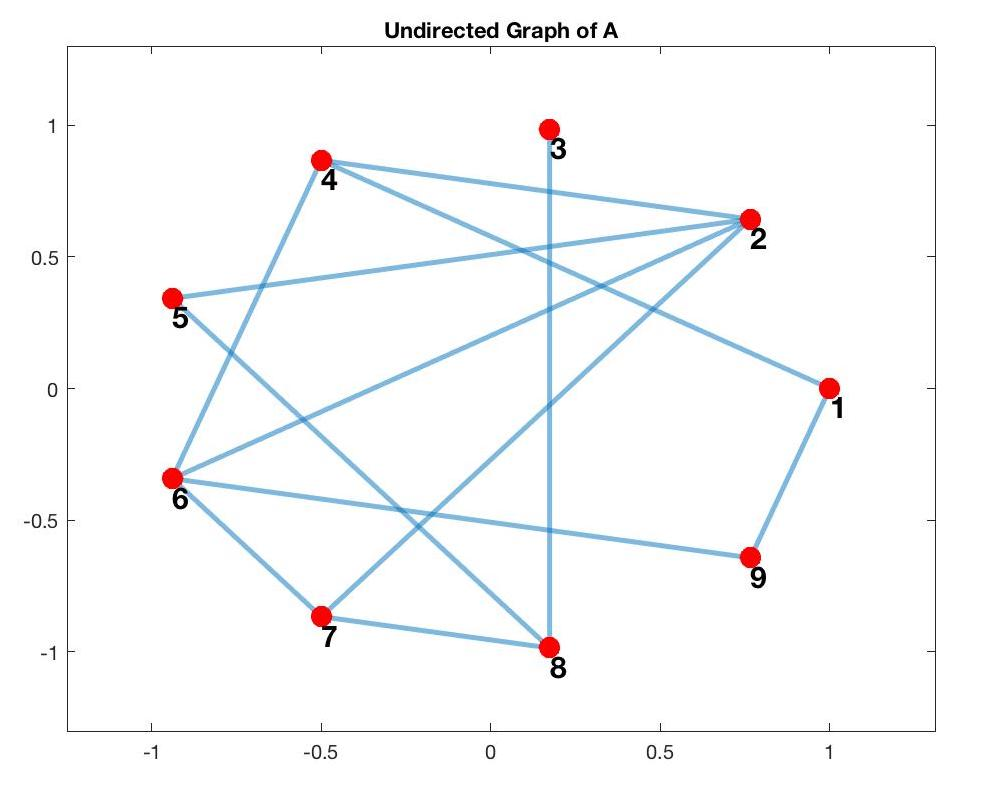
\includegraphics[scale=.3]{Undirected_Graph_of_A.jpg}
\caption{Undirected Graph Associated with A}
\end{figure}


\item[(b)] Use the minimum degree algorithm to reorder the matrix.\\

\begin{figure}[H]
\center
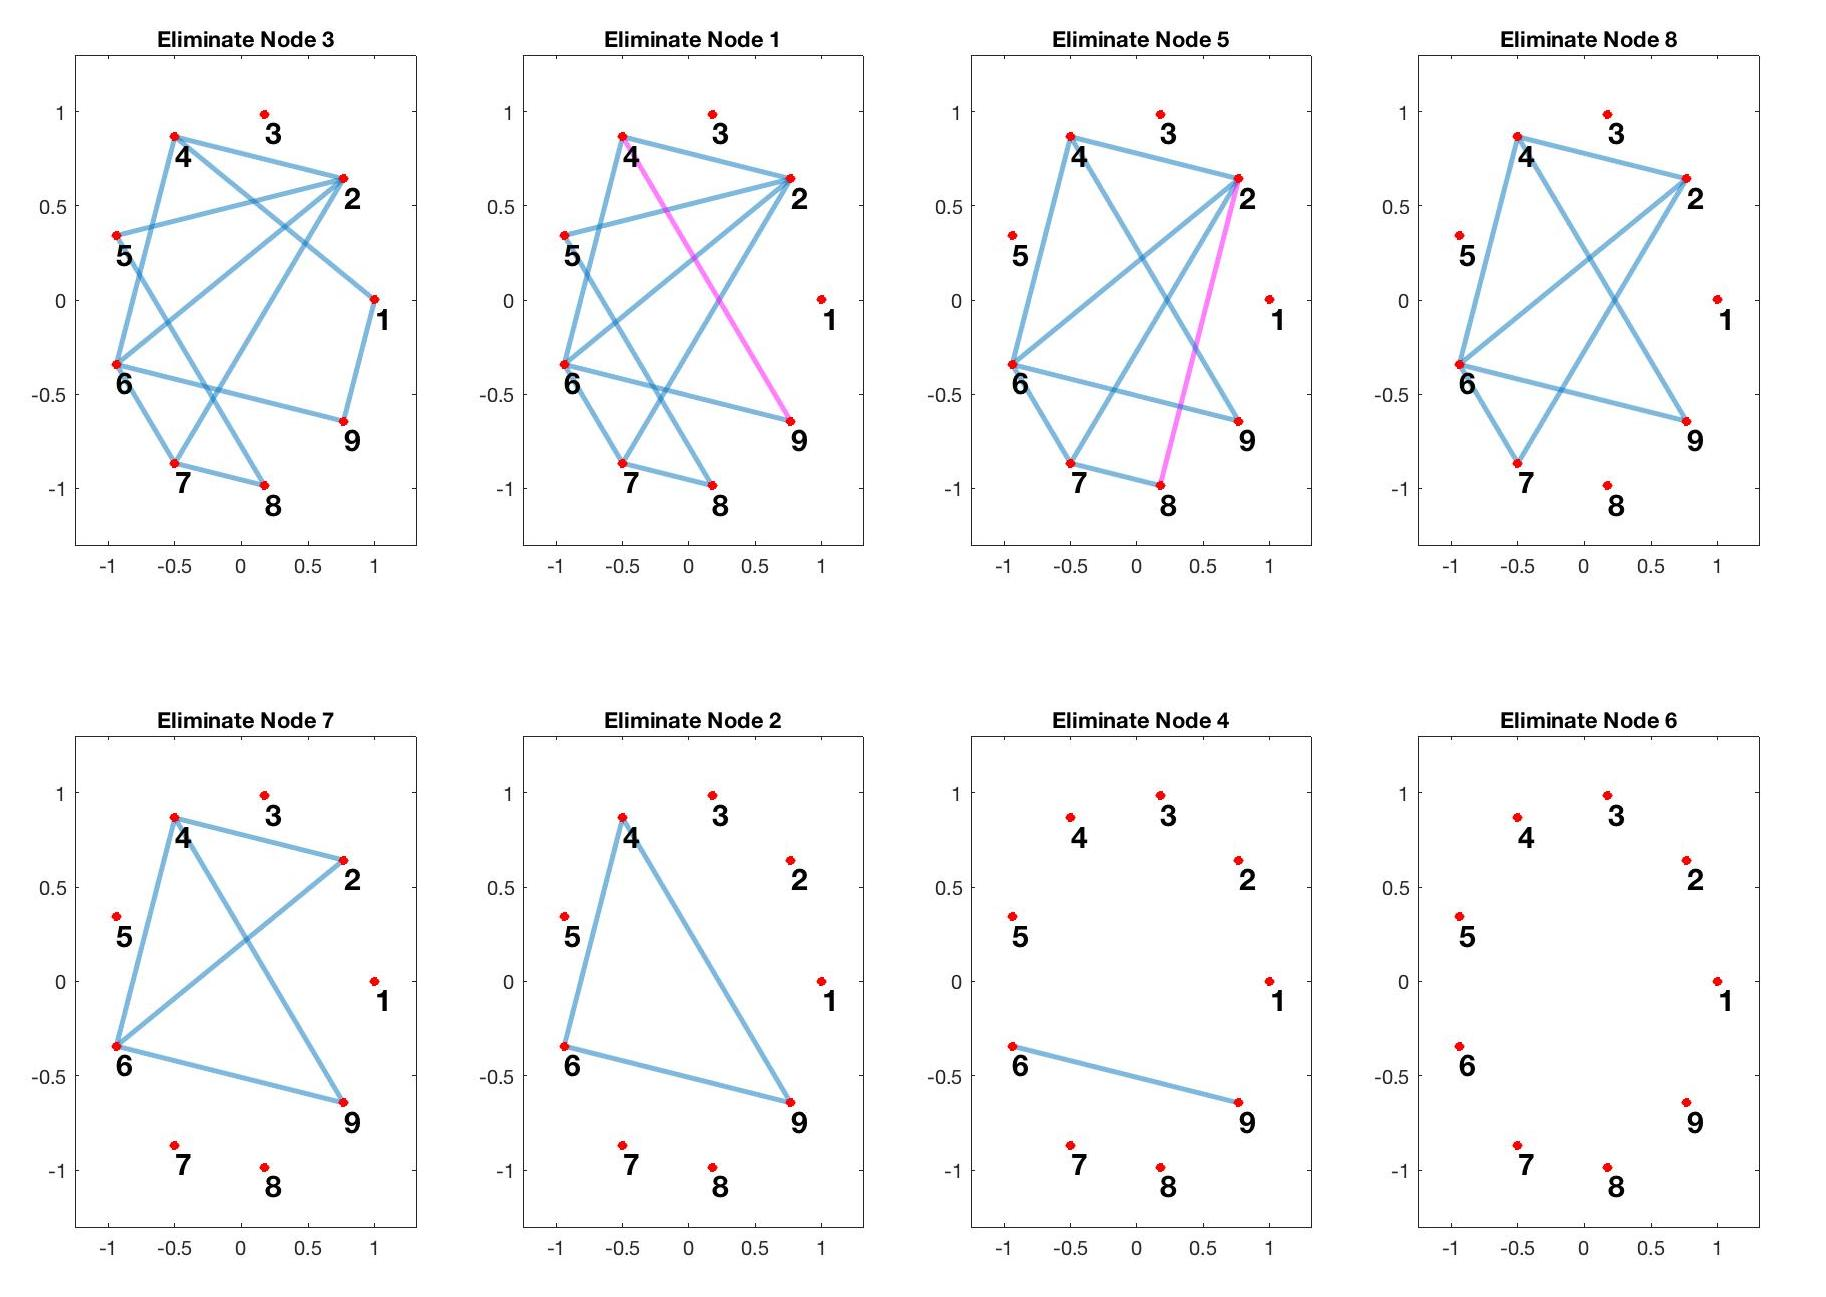
\includegraphics[scale=.23]{Undirected_Elimination_Graphs.jpg}
\caption{Undirected Graphs Corresponding to the Elimination of Minimal Degree Nodes}
\end{figure}

Note that in the above figure, red dots are nodes, blue lines indicate links between nodes, and pink lines indicate fill-in links created by the elimination of a node with adjacent connections.\\

By keeping track of the order in which we remove the nodes of minimal degree, we can determine the reordering of the matrix $A$.\\
So, based on the above undirected graphs, we can see that the reordering of the rows and columns of matrix $A$ corresponds to     $\begin{bmatrix}
 3 & 1 & 5 & 8 & 7 & 2 & 4 & 6 & 9 \\
\end{bmatrix}.$\\
\qed

\item[(c)] Show the sparsity structure of the sparse Cholesky factor $L$ of $P^TAP$, where $P$ is the permutation matrix corresponding to the minimum-degree ordering determined in part (b).\\

From the reordering determined in part (b), we can construct the permutation matrix $P$ as follows:
$$P = \begin{bmatrix}
0 & 1 & 0 & 0 & 0 & 0 & 0 & 0 & 0 \\
0 & 0 & 0 & 0 & 0 & 1 & 0 & 0 & 0 \\
1 & 0 & 0 & 0 & 0 & 0 & 0 & 0 & 0 \\
0 & 0 & 0 & 0 & 0 & 0 & 1 & 0 & 0 \\
0 & 0 & 1 & 0 & 0 & 0 & 0 & 0 & 0 \\
0 & 0 & 0 & 0 & 0 & 0 & 0 & 1 & 0 \\
0 & 0 & 0 & 0 & 1 & 0 & 0 & 0 & 0 \\
0 & 0 & 0 & 1 & 0 & 0 & 0 & 0 & 0 \\
0 & 0 & 0 & 0 & 0 & 0 & 0 & 0 & 1 \\
\end{bmatrix}$$

In part (b), there were 2 fill-in edges inserted between 4 $\&$ 9, and 2 $\&$ 8.  So now, we can rewrite $A$ including these fill-in elements in location $(2,8), (4,9), (8,2), (9,4)$.
$$\tilde{A} = \begin{bmatrix}
* & 0 & 0 & * & 0 & 0 & 0 & 0 & * \\
0 & * & 0 & * & * & * & * & \color{blue}\circlesign{*} & 0 \\
0 & 0 & * & 0 & 0 & 0 & 0 & * & 0 \\
* & * & 0 & * & 0 & * & 0 & 0 & \color{blue}\circlesign{*} \\
0 & * & 0 & 0 & * & 0 & 0 & * & 0 \\
0 & * & 0 & * & 0 & * & * & 0 & * \\
0 & * & 0 & 0 & 0 & * & * & * & 0 \\
0 & \color{blue}\circlesign{*} & * & 0 & * & 0 & * & * & 0 \\
* & 0 & 0 & \color{blue}\circlesign{*} & 0 & * & 0 & 0 & * \\
\end{bmatrix},$$

where $\color{blue}\circlesign{*}$ denotes a fill-in element.\\

Now, we can apply $P^T$ and $P$ to $\tilde{A}$ to permute the rows and columns corresponding to the reordering that we determined in part (b).  So,
$$P^T\tilde{A}P = \begin{bmatrix}
* & 0 & 0 & * & 0 & 0 & 0 & 0 & 0 \\
0 & * & 0 & 0 & 0 & 0 & * & 0 & * \\
0 & 0 & * & * & 0 & * & 0 & 0 & 0 \\
* & 0 & * & * & * & \color{blue}\circlesign{*} & 0 & 0 & 0 \\
0 & 0 & 0 & * & * & * & 0 & * & 0 \\
0 & 0 & * & \color{blue}\circlesign{*} & * & * & * & * & 0 \\
0 & * & 0 & 0 & 0 & * & * & * & \color{blue}\circlesign{*} \\
0 & 0 & 0 & 0 & * & * & * & * & * \\
0 & * & 0 & 0 & 0 & 0 & \color{blue}\circlesign{*} & * & * \\
\end{bmatrix}.$$

Now, since we are looking for $L$ such that $P^T\tilde{A}P = LL^T$, and since $P^T\tilde{A}P$ is symmetric, then we can see that the lower triangular matrix $L$ is the lower triangular part of the above matrix.  So, we can see the sparsity structure of the Cholesky factor $L$ is:
$$L = \begin{bmatrix}
* & 0 & 0 & 0 & 0 & 0 & 0 & 0 & 0 \\
0 & * & 0 & 0 & 0 & 0 & 0 & 0 & 0 \\
0 & 0 & * & 0 & 0 & 0 & 0 & 0 & 0 \\
* & 0 & * & * & 0 & 0 & 0 & 0 & 0 \\
0 & 0 & 0 & * & * & 0 & 0 & 0 & 0 \\
0 & 0 & * & \color{blue}\circlesign{*} & * & * & 0 & 0 & 0 \\
0 & * & 0 & 0 & 0 & * & * & 0 & 0 \\
0 & 0 & 0 & 0 & * & * & * & * & 0 \\
0 & * & 0 & 0 & 0 & 0 & \color{blue}\circlesign{*} & * & * \\
\end{bmatrix}.$$
\qed


\end{itemize}


\bigskip\bigskip
\noindent
\textbf{Problem 3:} Suppose that at the beginning of the $k$-th step of sparse $LU$ factorization, the matrix $U^{(k)}$ has the given sparsity structure.  Moreover, the nonzero entries $u_{il} \neq 0$ of $U^{(k)}$ are assumed to satisfy
$$\min_{i,l: u_{il}\neq 0} |u_{il}| \geq \frac{1}{3} \max_{i,l} |u_{il}|.$$\\

\begin{itemize}

\item[(a)] Determine the number of fill-in elements and their location if the $k$-th step is performed without pivoting.\\

After the $k$-th step of $LU$ factorization, we get $U^{(k+1}$ is:
$$U^{(k+1)} = \begin{bmatrix}
* & * & * & 0 & * & 0 & 0 & 0 & 0 & 0 & 0 \\
* & \color{blue}\circlesign{*} & \color{blue}\circlesign{*} & 0 & \color{blue}\circlesign{*} & 0 & 0 & 0 & 0 & 0 & * \\
0 & 0 & 0 & * & * & 0 & 0 & 0 & * & * & 0 \\
* & \color{blue}\circlesign{*} & \color{blue}\circlesign{*} & 0 & \color{blue}\circlesign{*} & * & 0 & 0 & * & 0 & 0 \\
* & \color{blue}\circlesign{*} & \color{blue}\circlesign{*} & 0 & \color{blue}\circlesign{*} & 0 & * & * & 0 & 0 & 0 \\
0 & 0 & 0 & * & 0 & 0 & 0 & 0 & 0 & * & * \\
* & \color{blue}\circlesign{*} & * & * & \color{blue}\circlesign{*} & * & 0 & 0 & 0 & * & 0 \\
0 & * & 0 & 0 & 0 & * & 0 & 0 & 0 & * & 0 \\
0 & 0 & 0 & 0 & 0 & 0 & * & * & 0 & * & 0 \\
* & \color{blue}\circlesign{*} & \color{blue}\circlesign{*} & * & \color{blue}\circlesign{*} & 0 & 0 & * & 0 & 0 & 0 \\
* & \color{blue}\circlesign{*} & \color{blue}\circlesign{*} & 0 & \color{blue}\circlesign{*} & * & 0 & 0 & 0 & 0 & * \\
\end{bmatrix},$$

where $\color{blue}\circlesign{*}$ denotes a fill-in element.\\

There are 17 fill-in elements at locations: $(2,2), (2,3), (2,5), (4,2), (4,3), (4,5),$\\
$(5,2), (5,3), (5,5), (7,2), (7,5), (10,2), (10,3), (10,5), (11,2), (11,3),(11,5)$.
\qed

\item[(b)] Determine the number of fill-in elements and their location if the $k$-th step is performed with a pivot element determined via the practice Markowitz criterion (with parameter $\alpha = 0.1$) presented in class.\\

Since we are given that:
$$\min_{i,l: u_{il}\neq 0} |u_{il}| \geq \frac{1}{3} \max_{i,l} |u_{il}|,$$

then,
\begin{align}
|u_{il} &\geq \alpha \max_{j \geq k} |u_{ij}| \nonumber \\
|u_{il} &\geq 0.1 \max_{j \geq k} |u_{ij}| \nonumber
\end{align}

is satisfied by all nonzero entries $u_{il}$ of $U^{(k)}$.  So, in order to  determine which entry of $U^{(k)}$ should be used as the pivot for the $k$-th step of $LU$ factorization, we just need to find the entry corresponding to the row and column with the lowest number of nonzero entries.  So, we can label the matrix $U^{(k)}$ as follows, where the number above a column or next to a row denotes the number of nonzero entries in that column or row.\\
$$U^{(k)} = \bbordermatrix{
r_i\backslash c_l & 7 & \color{blue} 2 & 2 & 4 & 2 & 4 & 2 & 3 & 2 & 5 & \color{red} 3 \cr
4 & * & * & * & 0 & * & 0 & 0 & 0 & 0 & 0 & 0 \cr
\color{red} 2 & * & \color{purple} 0 & 0 & 0 & 0 & 0 & 0 & 0 & 0 & 0 & \color{red}* \cr
4 & 0 & 0 & 0 & * & * & 0 & 0 & 0 & * & * & 0 \cr
3 & * & 0 & 0 & 0 & 0 & * & 0 & 0 & * & 0 & 0 \cr
3 & * & 0 & 0 & 0 & 0 & 0 & * & * & 0 & 0 & 0 \cr
3 & 0 & 0 & 0 & * & 0 & 0 & 0 & 0 & 0 & * & * \cr
5 & * & 0 & * & * & 0 & * & 0 & 0 & 0 & * & 0 \cr
3 & 0 & * & 0 & 0 & 0 & * & 0 & 0 & 0 & * & 0 \cr
3 & 0 & 0 & 0 & 0 & 0 & 0 & * & * & 0 & * & 0 \cr
3 & * & 0 & 0 & * & 0 & 0 & 0 & * & 0 & 0 & 0 \cr
3 & * & 0 & 0 & 0 & 0 & * & 0 & 0 & 0 & 0 & * \cr}$$


We can see, that row 2 ({\color{red}red 2}) and column 2 ({\color{blue}blue 2}) both have the lowest number of nonzero entries, and the lowest index numbers.  However, entry $(2,2)$ is zero ({\color{purple}purple 0}), so it cannot be used as a pivot.  In class, we stated that in the case where we need a tie-breaker, as we do now, then we first choose the smallest $i$, and then choose the smallest $l$.  i.e., our priority is to have the smallest index for the rows, and then we choose the smallest index of the columns that satisfies our conditions.\\

So, we determine that the pivot entry corresponds to the entry in row 2 ({\color{red}red 2}) and column 11 ({\color{red}red 3}).  So, the pivot element ({\color{red}*}) is in location $(2,9)$ of matrix $U^{(k)}$.  Which, minimizes:
\begin{align}
(r_i - 1)(c_l - 1) &= (r_2 - 1)(c_9 - 1) \nonumber \\
&= (2 - 1)(3 - 1) \nonumber \\
&= 2 \nonumber
\end{align}

Thus, 2 is the maximum number of fill-in elements produced by the $k$-th step of $LU$ factorization with pivoting.\\

Now, in order to determine the location of the fill-in elements, we can reorder matrix $U^{(k)}$ to put the pivot element in the top left corner by swapping rows 2 $\&$ 9, and columns 2 $\&$ 9, and perform the $k$-th step of $LU$ factorization as follows:
$$\tilde{U^{(k+1)}} = \begin{bmatrix}
\color{red}* & 0 & 0 & 0 & 0 & 0 & 0 & 0 & 0 & 0 & * \\
0 & * & * & 0 & * & 0 & 0 & 0 & 0 & 0 & * \\
0 & 0 & 0 & * & * & 0 & 0 & 0 & * & * & 0 \\
0 & 0 & 0 & 0 & 0 & * & 0 & 0 & * & 0 & * \\
0 & 0 & 0 & 0 & 0 & 0 & * & * & 0 & 0 & * \\
* & 0 & 0 & * & 0 & 0 & 0 & 0 & 0 & * & \color{blue}\circlesign{*} \\
0 & 0 & * & * & 0 & * & 0 & 0 & 0 & * & * \\
0 & * & 0 & 0 & 0 & * & 0 & 0 & 0 & * & 0 \\
0 & 0 & 0 & 0 & 0 & 0 & * & * & 0 & * & 0 \\
0 & 0 & 0 & * & 0 & 0 & 0 & * & 0 & 0 & * \\
* & 0 & 0 & 0 & 0 & * & 0 & 0 & 0 & 0 & * \\
\end{bmatrix},$$

where $\color{blue}\circlesign{*}$ denotes a fill-in element.\\

So, we can see that there is actually only 1 fill-in element produced by the $k$-th step of $LU$ factorization with pivoting, and its location is entry $(6,11)$.
\qed
\end{itemize}



\bigskip\bigskip
\noindent
\textbf{Problem 4:} \\

\begin{itemize}

\item[(a)] Let $L \in \R^{n\times n}$ be a unit lower-triangular matrix given in Matlab's sparse matrix format.  Employ Matlab's "find" command to write an efficient Matlab function that generates integer vectors $J$ and $I$ and a real vector $V_L$ that store the strictly lower-triangular part of $L$ in compressed sparse column format.\\  
To test your function, first apply it to the matrix $L$ provided in $\text{"small\_ex.mat"}$ and print out $J$, $I$, and $V_L$.  then apply your function to the matrix $L$ provided in $\text{"large\_ex.mat"}$.\\

\lstset{language=matlab,frame=single}
\begin{lstlisting}[caption= Generate $J\text{,}$ $I\text{,}$ and $V_L$ for Sparse Lower-Triangular Matrix]
function [JL,IL,VL] = SparseLowerTri(L)

Lt = tril(L,-1);
[JL, KL, VL] = find(Lt);

IL(1) = 1;

for i = 2:size(Lt,2)+1
   countL = nnz(Lt(:,i-1));
   IL(i) = IL(i-1) + countL;
end
IL = transpose(IL);
end
\end{lstlisting}

Using the above function for $L$ given in $\text{small\_ex.mat}$, we get the following results for $J$, $I$, and $V_L$:\\
$$J = \begin{bmatrix} 
3\\
     4\\
     9\\
     4\\
     5\\
     8\\
     9\\
     5\\
     7\\
     8\\
     6\\
     7\\
     8\\
     9\\
     8\\
     9\\
     7\\
     8\\
     9\\
     8\\
    10\\
\end{bmatrix}, I = \begin{bmatrix}
1\\
     4\\
     8\\
    11\\
    15\\
    17\\
    20\\
    21\\
    22\\
    22\\
    22\\
\end{bmatrix}, V_L = \begin{bmatrix}
8.127286465304295e-01\\
     2.578478773046358e-01\\
    -7.969322223753756e-01\\
    -8.907667695526849e-01\\
     2.565826406430549e-03\\
    -1.365576562315056e-01\\
     9.951206990243782e-01\\
    -2.869666020396466e-02\\
     7.888955111347864e-01\\
    -7.249068104658705e-01\\
     8.547124499962497e-01\\
     8.349876648322339e-01\\
     4.271480231886315e-01\\
     2.366747672438800e-01\\
     8.720546533795395e-01\\
    -7.504519186790148e-01\\
     2.929548648516276e-01\\
     6.663039713385901e-01\\
    -2.034355435624491e-01\\
     6.704410209562610e-01\\
     1.045232337167099e-01\\
\end{bmatrix}$$



\begin{table}[H]
\centering
\renewcommand{\arraystretch}{1.3}
\begin{tabular}{| c | c |}
\hline
Result &  Value\\
\hline 

$I_{50000}$ &  326956 \\

$I_{100000}$ & 1662354 \\

$I_{150000}$ & 4566327 \\

$I_{200000}$ &  12266446 \\

$I_{250000}$ & 15263327 \\
\hline
\end{tabular}
\caption{Select I values for the matrix L given in $\text{large\_ex.mat}$.}
\end{table} 
\qed

\item[(b)] Let $U \in\R^{n\times n}$ be a nonsingular upper-triangular matrix given in Matlab's sparse matrix format.  Employ Matlab's "find" command to write an efficient Matlab function that generates integer vectors $J$ and $I$ and a real vector $V_U$ that store $U$ in compressed sparse column format.\\  
To test your function, first apply it to the matrix $L$ provided in $\text{"small\_ex.mat"}$ and print out $J$, $I$, and $V_U$.  then apply your function to the matrix $L$ provided in $\text{"large\_ex.mat"}$.\\

\lstset{language=matlab,frame=single}
\begin{lstlisting}[caption= Generate $J\text{,}$ $I\text{,}$ and $V_U$ for Sparse Upper-Triangular Matrix]
function [JU,IU,VU] = SparseUpperTri(U)

[JU, KU, VU] = find(U);

IU(1) = 1;

for i = 2:size(U,2)+1
   countU = nnz(U(:,i-1));
   IU(i) = IU(i-1) + countU;
end
IU = transpose(IU);
end
end
\end{lstlisting}

Using the above function for $U$ given in $\text{small\_ex.mat}$, we get the following results for $J$, $I$, and $V_U$:\\
$$J = \begin{bmatrix} 
1\\
     2\\
     1\\
     3\\
     1\\
     2\\
     4\\
     2\\
     3\\
     5\\
     4\\
     6\\
     3\\
     4\\
     6\\
     7\\
     2\\
     3\\
     4\\
     5\\
     6\\
     7\\
     8\\
     1\\
     2\\
     4\\
     5\\
     6\\
     9\\
     8\\
    10\\
\end{bmatrix}, I = \begin{bmatrix}
1\\
     2\\
     3\\
     5\\
     8\\
    11\\
    13\\
    17\\
    24\\
    30\\
    32\\
\end{bmatrix}, V_U = \begin{bmatrix}
-7.227965685152800e-01\\
     1.764187707789873e-01\\
    -2.676863990901244e-01\\
     6.135190893222113e-01\\
     7.561571552311852e-03\\
    -2.081132255329154e-02\\
     7.540974467700878e-01\\
    -2.937163741220890e-01\\
    -1.011128868565034e-01\\
     9.270605736868538e-01\\
    -9.154044041709144e-01\\
     9.459166682812694e-01\\
    -6.215863137552480e-01\\
     3.342406000801499e-01\\
     1.728792293578358e-01\\
     3.502248328102306e-01\\
    -2.779559016106783e-01\\
     2.405568541421710e-01\\
     6.223017702005704e-01\\
    -9.614850451717172e-01\\
    -8.322529834342003e-01\\
     9.496033343697807e-01\\
     3.026990648307066e-01\\
    -5.375243676712955e-01\\
    -1.930177137508202e-01\\
    -7.559589634957409e-01\\
    -4.631223572054337e-01\\
    -4.843076597747906e-01\\
    -3.366695225147414e-01\\
    -6.955319742741071e-01\\
    -3.039846805677731e-01\\
\end{bmatrix}$$


\begin{table}[H]
\centering
\renewcommand{\arraystretch}{1.3}
\begin{tabular}{| c | c |}
\hline
Result &  Value\\
\hline 

$I_{50000}$ &  209763 \\

$I_{100000}$ & 1441841 \\

$I_{150000}$ & 4084326 \\

$I_{200000}$ &  14906853 \\

$I_{250000}$ & 17772343 \\
\hline
\end{tabular}
\caption{Select I values for the matrix U given in $\text{large\_ex.mat}$.}
\end{table} 
\qed

\item[(c)] Write two Matlab functions that solve systems of linear equations with unit lower-triangular coefficient matrices $L$ and nonsingular upper-triangular coefficient matrices $U$, respectively.  Here, $L$ and $U$ are given in the compressed sparse column format produced as output of your Matlab functions from (a) and (b).\\
To test your functions, first use them to solve the two triangular systems
$$Lc = b \text{   and   } Ux = c,$$
where $L$, $U$, and $b$ are provided in $\text{"small\_ex.mat"}$, and print out x.\\
Then use your functions to solve the systems, where $L$, $U$, and $b$ are provided in $\text{"large\_ex.mat"}$.\\

\lstset{language=matlab,frame=single}
\begin{lstlisting}[caption= Function to Solve $\text{Lc = b}$]
function c = Lsolve(IL,JL,VL,b)

c = b;

for k = 2:length(IL)-1
    indL = IL(k-1):IL(k) - 1;
    rL = JL(indL);
    c(rL) = c(rL) - VL(indL)*c(k-1);
end
end
\end{lstlisting}
\newpage
\lstset{language=matlab,frame=single}
\begin{lstlisting}[caption= Function to Solve $\text{Ux = c}$]
function x = Usolve(IU, JU, VU, c)

x = c;
n = length(c);

for j = length(IU)-1:-1:1
    indU = IU(j):IU(j+1) - 1;
    rU = JU(indU);
    x(j) = x(j)/VU(indU(end));
    x(rU(1:end-1)) = x(rU(1:end-1)) - x(j)*VU(indU(1:end-1));
end
end
\end{lstlisting}

Using the $L$ solver and $U$ solver above for $L$ and $U$ given in $\text{small\_ex.mat}$, we get the following result for x:\\
$$x = \begin{bmatrix} 
-7.368997733798020e+00\\
    -3.412065799871883e+01\\
     2.493451030044967e+01\\
    -2.682899840821154e+01\\
    -9.180874775319783e+00\\
    -1.237568442840570e+01\\
     2.593887743663491e+01\\
    -6.717855384133224e+00\\
    -4.296837993924318e+00\\
    -1.097654778394844e+00\\

\end{bmatrix}$$


\begin{table}[H]
\centering
\renewcommand{\arraystretch}{1.3}
\begin{tabular}{| c | c |}
\hline
Result &  Value\\
\hline 

$x_{50000}$ &  -7.306985715493668e+04 \\

$x_{100000}$ & -5.686028360745258e+05 \\

$x_{150000}$ & 5.850981452463222e+04 \\

$x_{200000}$ &  -6.238599598901578e+04 \\

$x_{250000}$ & 4.381939017807725e+06 \\

\hline
\end{tabular}
\caption{Select x values for L and U given in $\text{large\_ex.mat}$.}
\end{table} 
\qed
\end{itemize}
\newpage
\bigskip\bigskip
\noindent
\textbf{Problem 5:} Write a Matlab program that uses Matlab's $LU$ factorization $\text{"lu(A, 'vector')"}$ and your functions for triangular solves with $L$ and $U$ from problem 4(c) to compute the solution of 
$$Ax = b,$$
where $A \in\R^{n\times n}$ is a nonsingular sparse matrix and $b \in\R^n$.\\
To test your program, use it to solve the linear system for the two cases provided in $\text{"large\_ex1.mat"}$ and $\text{"large\_ex2.mat"}$.  Run your program with and without scaling, and
\begin{itemize}
\item[(i)] without column reordering,
\item[(ii)] with column reordering given by $p_0 = \text{colamd}(A)$,
\item[(iii)] with column reordering given by $p_0 = \text{colperm}(A)$.
\end{itemize}

\lstset{language=matlab,frame=single}
\begin{lstlisting}[caption= Solving $\text{Ax = b}$ using LU Factorization with Optional Scaling/Reordering]
function [error,zerosL,zerosU] = LUfactSolve(mat,scale,perm,permType)

if mat == 1
    load('large_ex1.mat')
elseif mat == 2
    load ('large_ex2.mat')
end

if scale == 0 % no scaling
    if perm == 0 % no column reordering
        p0 = 1:size(A,1);
        Ap = A(:,p0);
        
    elseif perm == 1 % yes column reordering
            if permType == 1 % column reordering using colamd
                p0 = colamd(A);
                Ap = A(:,p0);
                
            elseif permType == 2 % column reordering using colperm
                p0 = colperm(A);
                Ap = A(:,p0);  
            end
    end
    [L,U,p,q] = lu(Ap, 'vector');
    n = length(p);
    bp = b(p);

    [JL,IL,VL] = SparseLowerTri(L);
    c = Lsolve(IL,JL,VL,bp);
    [JU,IU,VU] = SparseUpperTri(U);
    d = Usolve(IU, JU, VU, c);

    qi(q) = 1:n;
    p0i(p0) = 1:n;
    x = d(qi);
    x = x(p0i);
    
    % Print results
    zerosL = nnz(L)
    zerosU = nnz(U)
    error = norm(b-A*x)/(norm(b))
    x(10)
    x(100)
    x(1000)
    x(100000)
    x(200000)
    
elseif scale == 1 % yes scaling
    if perm == 0 % no column reordering
        p0 = 1:size(A,1);
        Ap = A(:,p0);
        
    elseif perm == 1 % yes column reordering
            if permType == 1 % column reordering using colamd
                p0 = colamd(A);
                Ap = A(:,p0);
                
            elseif permType == 2 % column reordering using colperm
                p0 = colperm(A);
                Ap = A(:,p0);  
            end
    end
    [L,U,p,q,D] = lu(Ap,'vector');
    n = length(p);
    bp = D\b;
    bp = bp(p);

    [JL,IL,VL] = SparseLowerTri(L);
    c = Lsolve(IL,JL,VL,bp);
    [JU,IU,VU] = SparseUpperTri(U);
    d = Usolve(IU, JU, VU, c);

    qi(q) = 1:n;
    p0i(p0) = 1:n;
    x = d(qi);
    x = x(p0i);

    zerosL = nnz(L)
    zerosU = nnz(U)
    error = norm(b-A*x)/(norm(b))
    x(10)
    x(100)
    x(1000)
    x(100000)
    x(200000)
end
end  
\end{lstlisting}

\underline{Results:}\\

\begin{table}[H]
\centering
\renewcommand{\arraystretch}{1.3}
\begin{small}
\begin{tabular}{| c | c | c | c |}
\hline
$\textbf{large\_ex1.mat}$ &  (i) without reordering & (ii) reordering with colamd & (iii) reordering with colperm \\
\hline 
Scaling & No & No & No \\
\hline
nnz(L) & 48168142 & 48108479 & 41297742  \\
nnz(U) & 75157638 & 102737914 & 81257904  \\
$\frac{||b-Ax||_2}{||b||_2}$  & 2.828029206810877e-12 & 1.067252484791601e-11 &  2.374530280936845e-14 \\
$x_{10}$   & 1.648659303717927e-01 & 1.648659350646021e-01 & 1.648659289786954e-01  \\
$x_{100}$   & -4.194092835197273e-03 & -4.194106916432453e-03 & -4.194114069996023e-03  \\
$x_{1000}$   & 5.925158962408246e-01 & 5.925158936996825e-01 & 5.925158865659367e-01  \\
$x_{100000}$   & 8.783706938513887e-01 & 8.783706934654961e-01 &  8.783706929290729e-01 \\
$x_{200000}$   & -5.072168967563331e-01 & -5.072168967582433e-01 &  -5.072168967566794e-01 \\
\hline
\end{tabular}
\end{small}
\caption{Results for solving $\text{Ax = b}$, with A given in $\text{large\_ex1.mat}$, without scaling.}
\end{table} 

\begin{table}[H]
\centering
\renewcommand{\arraystretch}{1.3}
\begin{small}
\begin{tabular}{| c | c | c | c |}
\hline
$\textbf{large\_ex1.mat}$ &  (i) without reordering & (ii) reordering with colamd & (iii) reordering with colperm \\
\hline 
Scaling & Yes & Yes & Yes \\
\hline
nnz(L) & 26072934 & 23088688 &  22964802 \\
nnz(U) & 41192037 & 37633034 &  33686073 \\
$\frac{||b-Ax||_2}{||b||_2}$  & 6.790398425331222e-14 & 8.116366886591767e-14 &  5.125021168696811e-14 \\
$x_{10}$   & 1.648659289863991e-01 & 1.648659289637153e-01 &  1.648659289574123e-01 \\
$x_{100}$   & -4.194114045751002e-03 & -4.194114088398794e-03 &  -4.194114092583480e-03 \\
$x_{1000}$   & 5.925158865881905e-01 & 5.925158865422410e-01 &  5.925158865519882e-01 \\
$x_{100000}$   & 8.783706932199181e-01 & 8.783706927193258e-01 &  8.783706921651186e-01 \\
$x_{200000}$   & -5.072168967578401e-01 & -5.072168967583730e-01 &  -5.072168967580768e-01 \\
\hline
\end{tabular}
\end{small}
\caption{Results for solving $\text{Ax = b}$, with A given in $\text{large\_ex1.mat}$, with scaling.}
\end{table} 

\begin{table}[H]
\centering
\renewcommand{\arraystretch}{1.3}
\begin{small}
\begin{tabular}{| c | c | c | c |}
\hline
$\textbf{large\_ex2.mat}$ & (i) without reordering & (ii) reordering with colamd & (iii) reordering with colperm \\
\hline
Scaling & No & No & No \\
\hline
nnz(L) & 31884425 &  27171660 & 31881221 \\
nnz(U) & 44449862  &  40375283 & 44458733 \\
$\frac{||b-Ax||_2}{||b||_2}$ &  1.714118657717020e-16 & 1.595032981960684e-16  & 1.688597557702839e-16 \\
$x_{10}$ & 2.458207514024446e-02  &  2.458207507012133e-02 & 2.458207506433907e-02 \\
$x_{100}$ & 5.605584815600856e-01  &  5.605584815592441e-01 & 5.605584815615668e-01 \\
$x_{1000}$ & 7.647364835453209e-01  & 7.647364831250530e-01  & 7.647364840121942e-01 \\
$x_{100000}$ &  -1.202680373676209e-01 &  -1.202680363917079e-01 & -1.202680387313903e-01 \\
$x_{200000}$ & 3.236492069061306e-01  & 3.236303034450640e-01  & 3.236818364053314e-01 \\
\hline
\end{tabular}
\end{small}
\caption{Results for solving $\text{Ax = b}$, with A given in $\text{large\_ex2.mat}$, without scaling.}
\end{table} 

\begin{table}[H]
\centering
\renewcommand{\arraystretch}{1.3}
\begin{small}
\begin{tabular}{| c | c | c | c |}
\hline
$\textbf{large\_ex2.mat}$ &  (i) without reordering & (ii) reordering with colamd & (iii) reordering with colperm \\
\hline 
Scaling & Yes & Yes & Yes \\
\hline
nnz(L)  & 30332527  & 26527116 & 30282854  \\
nnz(U)  & 43548033  & 39580786 & 43494197  \\
$\frac{||b-Ax||_2}{||b||_2}$   & 2.582444141156649e-14 & 6.751642453866837e-14  &  2.817217290485666e-14 \\
$x_{10}$ & 2.458207512732105e-02  & 2.458207514243743e-02 & 2.458207514934205e-02  \\
$x_{100}$ & 5.605584815617708e-01  & 5.605584815608536e-01 & 5.605584815617290e-01  \\
$x_{1000}$ & 7.647364836470724e-01  & 7.647364837608184e-01 & 7.647364838713968e-01  \\
$x_{100000}$ & -1.202680377157837e-01  & -1.202680374673154e-01 &  -1.202680383112680e-01 \\
$x_{200000}$ & 3.237236658894511e-01  & 3.236883480835579e-01 &  3.236958393916007e-01 \\
\hline
\end{tabular}
\end{small}
\caption{Results for solving $\text{Ax = b}$, with A given in $\text{large\_ex2.mat}$, with scaling.}
\end{table} 
\qed





\end{document}

% insert Matlab code
\lstset{language=matlab,frame=single}
\begin{lstlisting}[caption=]

\end{lstlisting}

% table template
\begin{table}[H]
\centering
\renewcommand{\arraystretch}{1.3}
\begin{tabular}{| c | c |}
\hline
Result &  Value\\
\hline 

\hline
\end{tabular}
\end{table} 



%9x9
$$\begin{bmatrix}
0 & 0 & 0 & 0 & 0 & 0 & 0 & 0 & 0 \\
0 & 0 & 0 & 0 & 0 & 0 & 0 & 0 & 0 \\
0 & 0 & 0 & 0 & 0 & 0 & 0 & 0 & 0 \\
0 & 0 & 0 & 0 & 0 & 0 & 0 & 0 & 0 \\
0 & 0 & 0 & 0 & 0 & 0 & 0 & 0 & 0 \\
0 & 0 & 0 & 0 & 0 & 0 & 0 & 0 & 0 \\
0 & 0 & 0 & 0 & 0 & 0 & 0 & 0 & 0 \\
0 & 0 & 0 & 0 & 0 & 0 & 0 & 0 & 0 \\
0 & 0 & 0 & 0 & 0 & 0 & 0 & 0 & 0 \\
\end{bmatrix}$$

%11x11
$$\begin{bmatrix}
0 & 0 & 0 & 0 & 0 & 0 & 0 & 0 & 0 & 0 & 0 \\
0 & 0 & 0 & 0 & 0 & 0 & 0 & 0 & 0 & 0 & 0 \\
0 & 0 & 0 & 0 & 0 & 0 & 0 & 0 & 0 & 0 & 0 \\
0 & 0 & 0 & 0 & 0 & 0 & 0 & 0 & 0 & 0 & 0 \\
0 & 0 & 0 & 0 & 0 & 0 & 0 & 0 & 0 & 0 & 0 \\
0 & 0 & 0 & 0 & 0 & 0 & 0 & 0 & 0 & 0 & 0 \\
0 & 0 & 0 & 0 & 0 & 0 & 0 & 0 & 0 & 0 & 0 \\
0 & 0 & 0 & 0 & 0 & 0 & 0 & 0 & 0 & 0 & 0 \\
0 & 0 & 0 & 0 & 0 & 0 & 0 & 0 & 0 & 0 & 0 \\
0 & 0 & 0 & 0 & 0 & 0 & 0 & 0 & 0 & 0 & 0 \\
0 & 0 & 0 & 0 & 0 & 0 & 0 & 0 & 0 & 0 & 0 \\
\end{bmatrix}$$

%border matrix with brackets template
$$M = \bbordermatrix{
 & x & y \cr
 A & 1 & 0 \cr
 B & 0 & 1 \cr}$$